
\section*{Implementation}

\subsection*{Project Structure}

One of the tasks that we have completed in this phase is to complete the design
of an structural framework that allows easy and incremental development of the
benchmarks. This section briefly describes the design.

Figure \ref{fig:package_structure} depicts the overview of the framework by mean
of the Java package structure. Figure \ref{fig:class_diagram} provides a closer
view at the organization of the classes related to the VectorAdd benchmark.

At a high level, we split the development of the graphical user interface (GUI),
from the development of each of the benchmarks, under the $GUI$ package and the
$parboil$ package in Figure \ref{fig:package_structure}, respectively. At this
stage, the GUI is simply to allow users to start running the benchmarks, and to 
display the status at the end of each benchmark, e.g., whether the benchmark has executed
successfully or failed. In the future, more features will be added, such as
display the progress of running the benchmarks, and the final scores of the
device. But we do not think that should be the focus of our development at this
moment.

The $parboil$ package is the core of the project. In this package, we
also identified the common functions, such as timing- and logging-related
functions, that are used across all the benchmarks. Those functions are further
grouped in classes, e.g., $Timer$ and $Logger$, and implemented in the $utils$
package. Each benchmark, e,g., $bfs$ or $cutcp$, is implemented in a separate
package under the $benchmark$ package. Figure \ref{fig:class_diagram} depicts
the class diagram of the VectorAdd benchmark. Other benchmarks have the same
class structure. In order to implement a benchmark, we just need to inherit for
the $ParboiBenchmark$ class, which layouts a common skeleton. For each
benchmark, we have to implement a class to read the input, for example
$VectorAddFileReader$ class in this case. Each computation kernel, e.g., for
Java, threaded Java, RenderScript, or OpenCL, is implemented in a separate
class, e.g., $VectorAddJava$, $VectorAddThreadedJava$, $VectorAddRS$, or
$VectorAddOpenCL$, respectively. These class inherits from the parent class of
the benchmark, which is the $VectorAddBenchmark$ in this case. This hierarchical
design maximize the code reuse between benchmarks, and between computation
kernel.





\begin{figure}[t!]
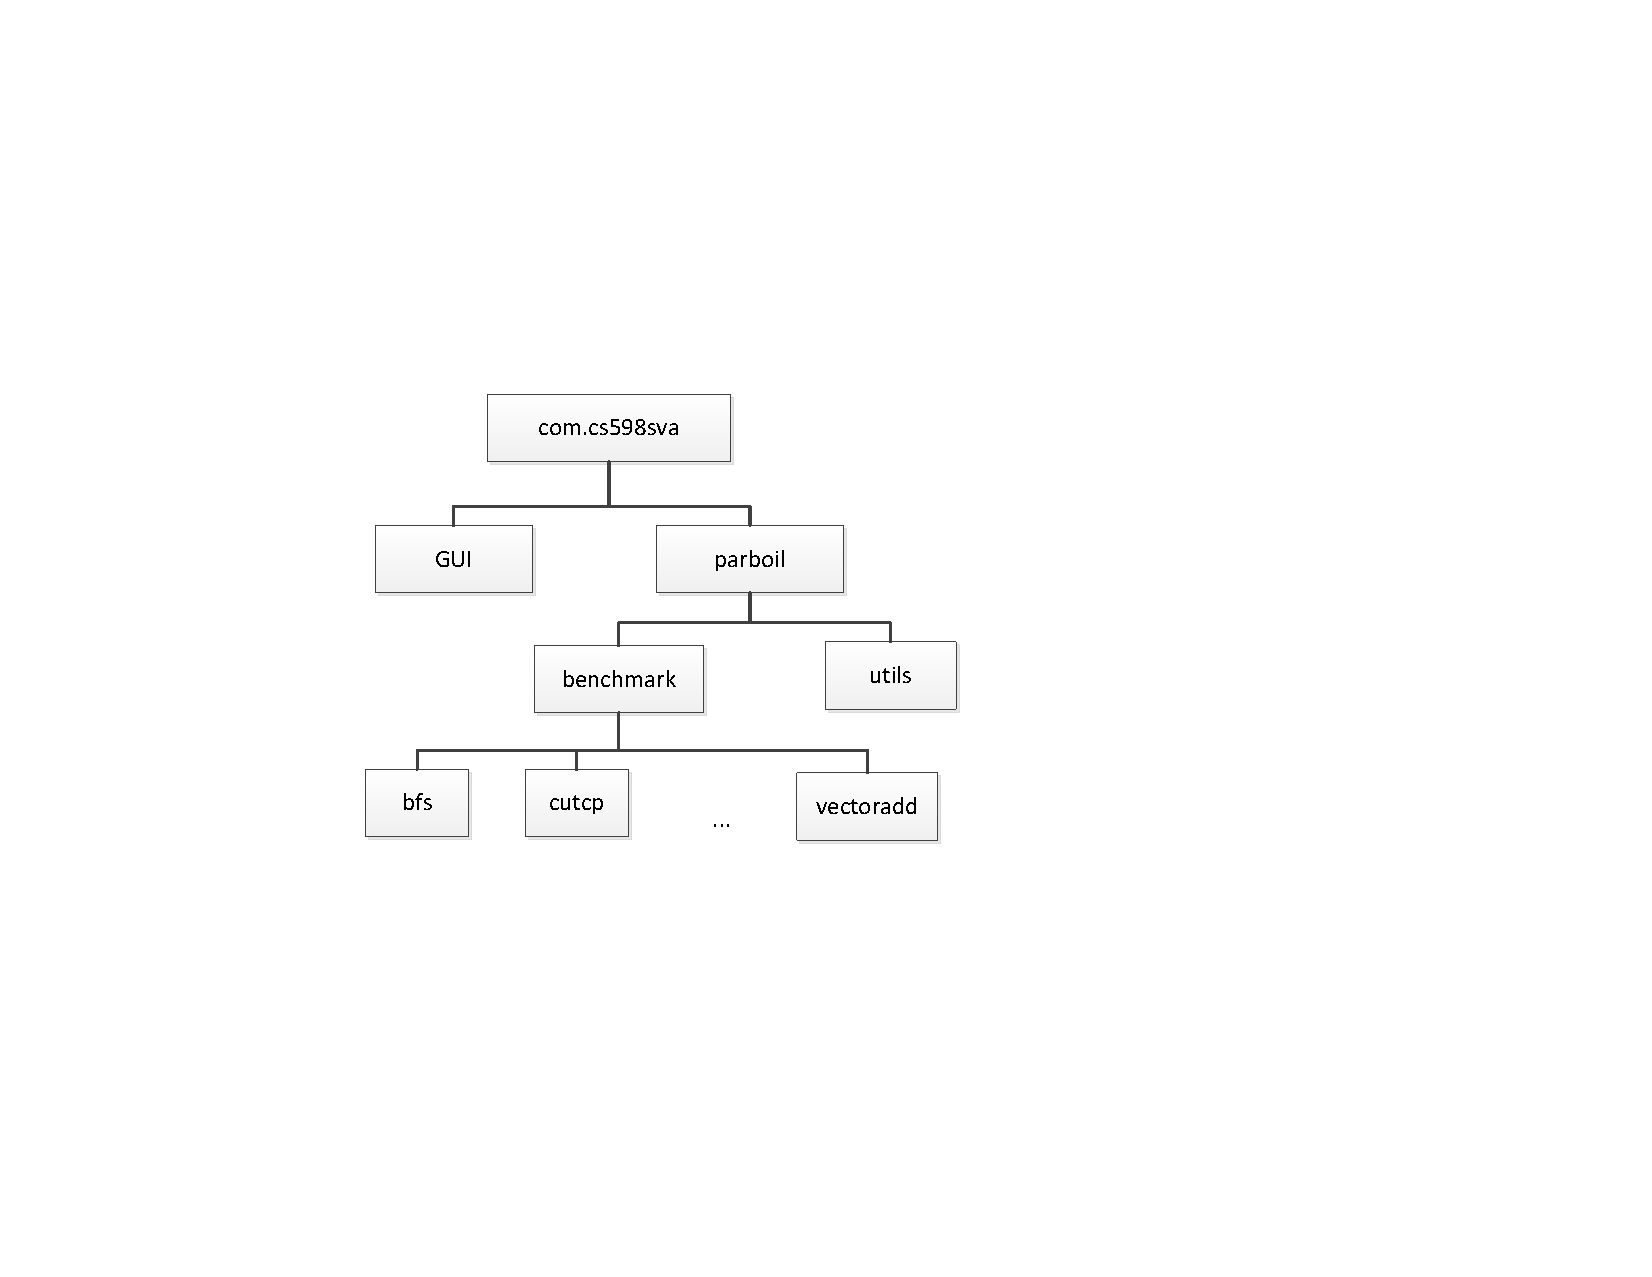
\includegraphics[scale=0.65]{figs/package_diagram.pdf}
\caption{RSBench Java package structure.}
\label{fig:package_structure}
\centering
\end{figure}


\begin{figure}[t!]
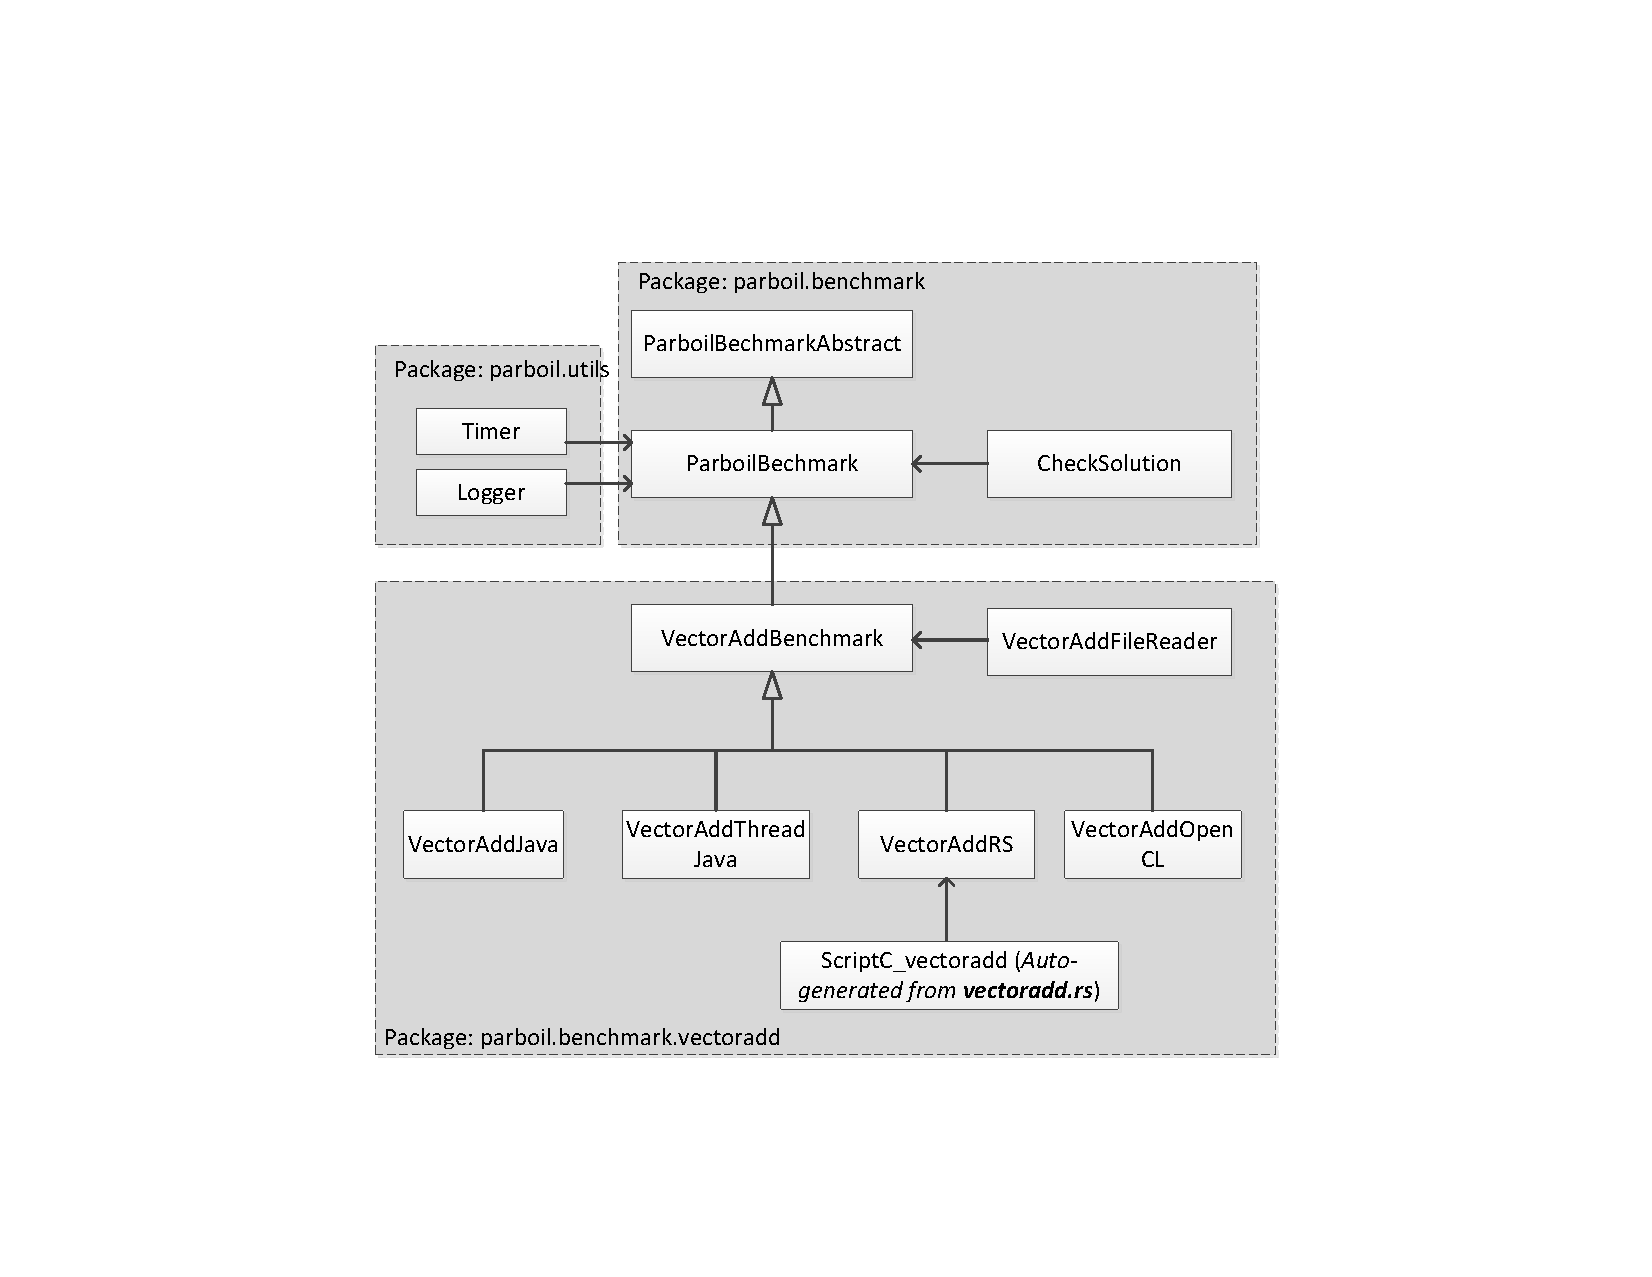
\includegraphics[scale=0.5]{figs/vectoradd_class_diagram.pdf}
\caption{Class diagram of the VectorAdd benchmark.}
\label{fig:class_diagram}
\centering
\end{figure}

\subsection*{Timer}



\subsection*{Output}


\begin{figure}[t!]
\begin{verbatim}
struct {
	string Type,
	string Hardware,
	string Benchmark,
	string Implementation,
	string Category,
	string Message,
	long StartTime,
	long EndTime,
	long ElapsedTime,
	string Data,
	string Date,
}
\end{verbatim}
\caption{Database Columns.}
\label{fig:database}
\centering
\end{figure}

Unlike Parboil, which outputs the times to {\tt stdout}, we output our data into a SQLite database.
This affords us a few things.
First, since data is outputed in the specified columns, we do not have to reparse the output data.
Second, timing information can be shared easily by copying the database.
Finally, we can store more than just timing information.

